\section{Implement Details}
\subsection{Proof Skeleton of Proposition~\ref{prop:smooth_randomization}}
\label{ap: Proof Skeleton of Propositio}
The parallel theorem establishes a bijective mapping between the rotational inertia w.r.t body frame origin $\mathbf{\bar{I}}$ and $\mathbf{\bar{I}}_{\text{C}}$
\begin{equation}
    \mathbf{\bar{I}}_{\text{C}} = \mathbf{\bar{I}} - m \ \textbf{S}(c)\textbf{S}(c)^{\top}.
\end{equation}

To obtain inertial parameters $\boldsymbol{\kappa}_{\text{link}}$ that corresponds to a physically plausible system~\cite{Traversaro2016manifolds,Wensing2018LMI}, we should have constraints:
\begin{equation}
\begin{aligned}
\label{eq: constraints}
        & m > 0~, \; D_{i} > 0, \\
        & D_1 + D_2 + D_3 > 2D_{i} \quad \forall i=1,2,3, \\[3pt]
\end{aligned}
\end{equation}
where $m > 0$, $D_1$, $D_2$ and $D_3$ are principal moments of inertia, such that $\mathbf{\bar{I}}_{\text{C}} = \mathbf{RDR^{\top}}$ with $\mathbf{D} = \text{diag}(D_1,D_2,D_3)$ and $\mathbf{R} \in \mathbf{SO}(3)$. Note that the triangle-inequality component of the constraint can be reformulated as:
\begin{equation}
\label{eq: constraint-temp-1}
    \frac{1}{2}\text{Tr}(\mathbf{\bar{I}}_{\text{C}}) \; > \; \lambda_\text{max}(\mathbf{\bar{I}}_{\text{C}})~,
\end{equation}
where $\text{Tr}(\cdot)$ is the trace operator, $\lambda_\text{max}(\cdot)$ extracts the maximum eigenvalue. Since $\mathbf{\bar{I}}_{\text{C}}$ is symmetric matrix, it must satisfy $\lambda_\text{max}(\mathbf{\bar{I}}_{\text{C}})\mathbf{I} \; \succeq \; \mathbf{\bar{I}}_{\text{C}}$, then Ineq. (\ref{eq: constraint-temp-1}) are equivalent to:
\begin{equation}
    \label{eq: }
    \mathbf{\Sigma}_{\text{C}} = \frac{1}{2}\text{Tr}(\mathbf{\bar{I}}_{\text{C}})\mathbf{I} -\mathbf{\bar{I}}_{\text{C}} \; \succ \; 0~.
\end{equation}
According to the parallel-axis theorem of pseudo-inertia~\cite{Wensing2018LMI}:
\begin{equation}\label{eq: parallel-axis}
    \mathbf{\Sigma}_{\text{C}} = \mathbf{\Sigma} - m\mathbf{cc}^{\top} = \mathbf{\Sigma} - \frac{1}{m}\mathbf{h}\mathbf{h}^{\top} \succ 0~,
\end{equation}
according to Schur complement, we can further consolidate the inertial constraints (\ref{eq: parallel-axis}) into a linear matrix inequality:
\begin{equation}
    \mathbf{J} =  \begin{bmatrix}
  \mathbf{\Sigma} & \mathbf{h}^{\top} \\
  \mathbf{h} & m
\end{bmatrix} \, \succ \, 0~,
\end{equation}
where $\mathbf{J} \in \mathbb{R}^{4 \times 4}$ is pseudo-inertia matrix of rigid body~\cite{Rucker2022smooth}, originally defined as the integral form:
\begin{equation}
    \mathbf{J} = \int_{V} \mathbf{qq}^{\top}\rho(\mathbf{x})dV~, \quad \textbf{q} = [\textbf{x}^{\top},1]^{\top},
\end{equation}
Therefore, obtaining a physically feasible set of inertial parameters only requires ensuring that the corresponding $\mathbf{J}$ is positive definite. A unique factorization by the Cholesky decomposition claims that a real symmetric matrix $\mathbf{J}$ is positive definite \textit{iff}. there exists a unique real nonsingular matrix $\mathbf{L}$ such that
\[
\mathbf{J} = \mathbf{L}\mathbf{L}^{\top}~,
\]
where $\mathbf{L}$ is upper-triangular with a positive diagonal.
Now we can physics-consistently randomize the link parameters, by perturbing the upper-triangular entries of $\mathbf{{L}}$:
\begin{equation}
    {\mathbf{J}}' = {\mathbf{L}}'{\mathbf{{L}}}'^{\top}~, \; \mathbf{{L}}' = \mathbf{{L}} + \boldsymbol{\epsilon}~, \; \boldsymbol{\epsilon}\sim \mathbf{\mathcal{D}}~,
\end{equation}
where $\mathbf{\mathcal{D}}$ is the noise distribution. To achieve an explainable randomization and provide geometric insight into the resulting link, instead of choosing a random distribution $\mathbf{\mathcal{D}}$, we model the perturbations as an affine transformation on the rigid bodies' geometry and scaling of the mass density:
\begin{equation}
    \begin{aligned}
    \label{eq: pseudo-inertia calculus-}
        \mathbf{J}^{'} & = \int_{V} \mathbf{Eqq}^{\top}\mathbf{E}^{\top}\beta^{2}\rho(\mathbf{x})dV \\
        & =\beta^{2} \mathbf{E}
        \underbrace{
        \int_{V} \mathbf{qq}^{\top}\rho(\mathbf{x})dV}_{\mathbf{J}}
        \mathbf{E}^{\top} \\
        & = \mathbf{U}\mathbf{J}\mathbf{U}^{\top}~,
    \end{aligned}
\end{equation}
where $\mathbf{U}=\beta\mathbf{E}$, $\mathbf{E}$ denotes the linear component of the affine transformation. 
% This result shows that transformations in pseudo-inertia space ${\mathbf{J}}'$ can be interpreted as arising from an affine deformation of a reference rigid body, combined with a uniform scaling of its mass density. 
Equation~(\ref{eq: pseudo-inertia calculus-}) can be rewritten as:
\begin{equation}
    \mathbf{L^{'}}\mathbf{L^{'\top}} = \mathbf{UL}\mathbf{L}^{\top}\mathbf{U}^{\top}~.
\end{equation}
from which it follows that $\mathbf{U} = \mathbf{L^{'}}\mathbf{L^{-1}}$ is a unique upper triangular matrix with positive diagonal entries, since both $\mathbf{L}$ and $\mathbf{L^{'}}$ are upper-triangular.
Thus, $\mathbf{U}$ can be parameterized using exponential mapping on the diagonal entries:
\begin{equation}
    \mathbf{U} = e^{\alpha} \begin{bmatrix}
  e^{d_1} &  s_{12} & s_{13} & t_1 \\
  0 &  e^{d_2} & s_{23} & t_2\\
  0 &  0 & e^{d_3} & t_3 \\
  0 &  0 & 0 & 1
\end{bmatrix}~,
\end{equation}
we finally obtain a bijecive mapping from original inertia to 10-dimensional explainable vector 
\[
    \theta_{\text{inert}} = [\alpha, d_1, d_2, d_3, s_{12}, s_{23}, s_{13}, t_1, t_2, t_3]^{\top} \in \mathbb{R}^{10}~.
\]
As a result, the random perturbation $\boldsymbol{\epsilon}$ applied at the Cholesky-factor level can be equivalently expressed as a perturbation in $\theta_{\text{inert}}$. The detailed $\theta_\text{inert}$ can be found in Appendix~\ref{tab:link_random_ranges}.


\subsection{Physical Interpretation of Morphological Randomization}
\label{ap: Physical Interpretation}
Based on the interpretation of $\mathbf{U}$ as a combination an affine transformation and a density scaling of reference rigid body, each parameter admits a clear physical meaning.
 
The parameters $d_1, d_2$ and $d_3$ correspond to stretching or compression of the reference rigid body along $x, y$ and $z$ axes, respectively, where $d_i > 0 \Rightarrow e^{d_i} > 1$ implies the stretching, and $d_i < 0 \Rightarrow e^{d_i} < 1$ denotes the compression. Importantly, this exponential formulation guarantees that the body never degenerates to zero thickness.

The shear parameters $s_{12}, s_{13}$ and $s_{23}$ induce shear deformations in the $xy, xz$ and $yz$ planes, respectively, without altering the volume of the object. 
The translation parameters $t_1, t_2$ and $t_3$ uniformly shift the center of mass of the reference rigid body along the $x, y$ and $z$ directions. Finally, the scalar parameters $\alpha$ controls a global scaling of the mass density $\rho$ by the factor $e^{2\alpha}$. 

In this work, we use the Unitree G1 (29 DoF) as a template, and the corresponding link and joint randomization ranges are listed in Tabs.~\ref{tab:link_random_ranges} and \ref{tab:joint_random_ranges}. All noise is sampled from a uniform distribution expected the rotation axis and actuation type. We denote revolute joint actuation as \textbf{R} and fixed joint actuation as \textbf{F}. The rotation axes $[a_x, a_y, a_z]$ of the three hip joints are randomly permuted rather than independently sampled. The orientation offsets $[\phi, \theta, \psi]$ are randomly generated with the constraint that their sum across the joint group is zero, ensuring no net orientation bias.
% 
\subsection{Policy Training}
\label{ap: Policy Training}
To achieve cross-embodiment learning, we employ either GCN or Transformer as representation-learning backbone. Joint-related observations in the policy input $o_t^{\pi}$ , including joint position $q_t$, joint velocities $\dot{q}_t$, actions $a_t$ and $I(t)$, are first mapped to canonical joint representation $\mathbf{q}_\text{global}$ via mapping function defined in \autoref{eq: global joint mapping function}. 

% \begin{figure}
%     \centering
%     \includegraphics[width=\linewidth]{images/adjacency_matrix.png}
%     \caption{\small \textbf{Embodiment adjacency matrix and hybrid-masking attention for the transformer.} The robot’s adjacency matrix is built from its kinematic chain, with entries set to 1 if two joints are directly connected. Three root nodes are defined according to anatomical function: a). the hip joint connect to the pelvis link. b). the waist joint connect to the pelvis link. c). the shoulder joint connect to the torso link.}
%     % \vspace{-7pt}
%     \label{fig:adjacence_matrix}
%     % \vspace{-10pt}
% \end{figure}

The resulting canonical representation is linearly projected, after which each joint node is processed by a node-specific learnable linear layer. This yields a sequence of $N_\text{max}$ canonical node embeddings. The remaining policy observations are concatenated into vectors $o_t^{g} = [w_t, g_t, c_t]$, which is later used in decoding stage to generate joint-level actions. 

Formally, the canonical node embedding $\mathbf{X}$ shared by both encoders.
For the Transformer encoder, positional embeddings are added, while the GCN encoder operates directly on $\mathbf{X}$.
\begin{equation}
    \mathbf{X} = \big[
    \phi_\theta^{1}(\mathbf{q}_\text{global}[1];\mathbf{W}_{\theta}^{1});
    \cdots; 
    \phi_\theta^{i}(\mathbf{q}_\text{global}[i];\mathbf{W}_{\theta}^{i})
    \big]~,
\end{equation}

where the $\phi_{\theta}(\cdot)$ is learnable embedding function parameters by weights $\mathbf{W}_{\theta} \in \mathbb{R}^{N \times D}$. 

\noindent\textbf{Encoder.}
We then apply a stack of GCN or transformer blocks as the encoder to selectively incorporate information beyond purely local kinematic neighborhood. For the GCN encoder, the input consists of the node embeddings $\textbf{X}$ (without positional embedding) together with the structural mask $\mathbf{M}=\mathbf{I}+\mathbf{A}$ (with self-loops):
\begin{equation}
    \textbf{Z} = \textbf{GCN}_\text{encoder}(\textbf{X, M})~,
\end{equation}

For the Transformer-based encoder, we adopt two types attention blocks: self-attention blocks (SAB) and masked-attention block (MAB), defined respectively as:
% , including two types of attention blocks: self-attention block (SAB) and masked-attention block (MAB):
\begin{equation}
\resizebox{0.95\linewidth}{!}{$
\begin{aligned}
\mathbf{MAB} &= \text{LayerNorm}(\mathbf{X}_{\text{pos}} + \text{MultiHead}(\mathbf{X}_{\text{pos}}, \mathbf{X}_{\text{pos}})), \\
\mathbf{SAB} &= \text{LayerNorm}(\mathbf{X}_{\text{pos}} + \text{MultiHead}(\mathbf{X}_{\text{pos}}, \mathbf{X}_{\text{pos}}, \mathbf{M}))
\end{aligned}
$}
\end{equation}
% with $\mathbf{I}_{n}$ denoting the identity matrix and $\mathbf{A}$ the adjacency matrix of the embodiment’s kinematic graph (Fig.~\ref{fig:adjacence_matrix}).
The hybrid-masking design is similarly to prior work~\cite{sferrazza2024bot}, in which the first encoder layer employs an SAB to enable global information exchange, while all subsequent layers use MABs to respect embodiment-specific structural constraints. Formally, the encoder is defined as
\begin{equation}
\begin{aligned}
    \textbf{Z} & = \mathbf{Encoder}(\mathbf{X}, \mathbf{M}) \\
               & = \mathbf{SAB} \circ \mathbf{MAB} \circ \cdots \mathbf{MAB}(\mathbf{X,M})~.
\end{aligned}
\end{equation}

\noindent\textbf{Action Decoder.}
The encoded node features $\textbf{Z}$ produced by either GCN or Transformer encoder are concatenated with the global context vector $o_t^{g}$ and the reconstructed privileged information $\mathbf{P}$ obtained from the learned state-estimation module. 
\begin{equation}
    \mathbf{P} = \mathbf{Estimator}(\text{Flatten}(\mathbf{Z}))
\end{equation}
where $\mathbf{Estimator}$ is state estimator trained by supervised learning~\cite{concurrent2022ral}. Joint-level actions are then decoded independently for each node:
\begin{equation}
\resizebox{0.95\linewidth}{!}{$
    \mathbf{a}_{\text{global}} = [\phi_{d}^{1}([\mathbf{Z}[1],\mathbf{P},o_t^{g}]; \mathbf{W}_{d}^{1}); ...\phi_{d}^{i}([\mathbf{Z}[i],\mathbf{P},o_t^{g}]; \mathbf{W}_{d}^{i})]~.
$}
\end{equation}
The resulting canonical action vector $\mathbf{a}_{\text{global}}$ is finally mapped back to the robot's physical joints through an embodiment-specific inverse mapping function:
\[
\operatorname{inv}(\phi_r): \mathbb{R}^{N_{\text{max}}} \rightarrow \mathbb{R}^{N_r}~.
\]

\input{tables/link_random_ranges}
\input{tables/joint_random_ranges}
\input{tables/robot_types}
\input{tables/rewards}

\input{tables/single_commands}

\subsection{Rewards Details}
The total rewards consists of three terms, including task rewards, behavior rewards and regularization rewards. Table \ref{tab:rewards} lists reward terms for \our.  The Contact-Swing Tracking reward is adopted from~\cite{xue2025hugwbc}.



\section{Extended Experiment}
\label{ap:extended exp}
\subsection{Metrics}
We evaluate ablation methods in Isaac Gym~\cite{makoviychu2021isaacgym} on the most and the policy performance is measured by two distinct metrics:

\noindent\textbf{Survival Rate}
$E_\text{surv}$ measures the trajectory survival rate over 1000 environments per episode. Non-termination is defined as the roll and pitch angle of the robot torso do not overturn beyond $60^\circ$.

\noindent\textbf{Average commands tracking error}
$E_\text{cmd}$ measures the average episodic tracking accuracy for a single command across 1000 environments. The metric is defined as the $L_1$ distance between the actual robot states and the command states. All commands are uniformly sampled within a predefined range.

Figure~\ref{fig:simulation_experiment} is visualization of simulation evaluation.

Figure~\ref{fig:embodiment data} is visualization of embodiment data generated by physics-consistent morphological randomization.

% We adopt the Unitree G1 as the sole template for data generation and augment it with three additional degrees of freedom in the head to maximize the diversity joint-space configurations. \our is trained exclusively on the embodied dataset described in Sec. \ref{sec: interpretable morphological randomization}. We then evaluate \our in simulation on 12 distinct humanoid robots and further validate its performance on 7 real-world robotic platforms, all of which differ substantially in physical properties and morphological structures. Among these platforms, the smallest platform weighs only 20~kg, whereas the largest full-size humanoid reaches 66~kg. The robots span a wide range of kinematic complexity, with the number of degrees of freedom varying from 18 to 31. 

% In the real-world experiments, all robots are connected within the same local area network and execute a shared policy, which synchronously generates robot-specific actions conditioned on each robot's state. The detailed physical properties of the robots and deployment procedures are provided in the Appendix~\ref{ap:extended exp}.

\input{tables/global_joint_index}

\subsection{Deployment Details}
We employ a modular and reusable deployment framework to simplify our sim-to-sim and sim-to-real experiment workflows across diverse embodiments~\cite{lin2026uniconunifiedefficientrobot}.
During multi-robot experiments, locomotion and manipulation commands are issued from one centralized workstation and synchronized with all robot participants over ZMQ-based communication channels, while each robot executes an identical locomotion policy on its own on-board computing device.
In addition, We combine the framework with existing IK solvers~\cite{carpentier2019pinocchio, pinocchioweb, pink} and teleoperation pipelines~\cite{Cheng2024OpenTeleVisionTW, unitreexrteleoperate} to enable whole-body, hardware-agnostic loco-manipulation.


\begin{figure*}[htbp]
\centering
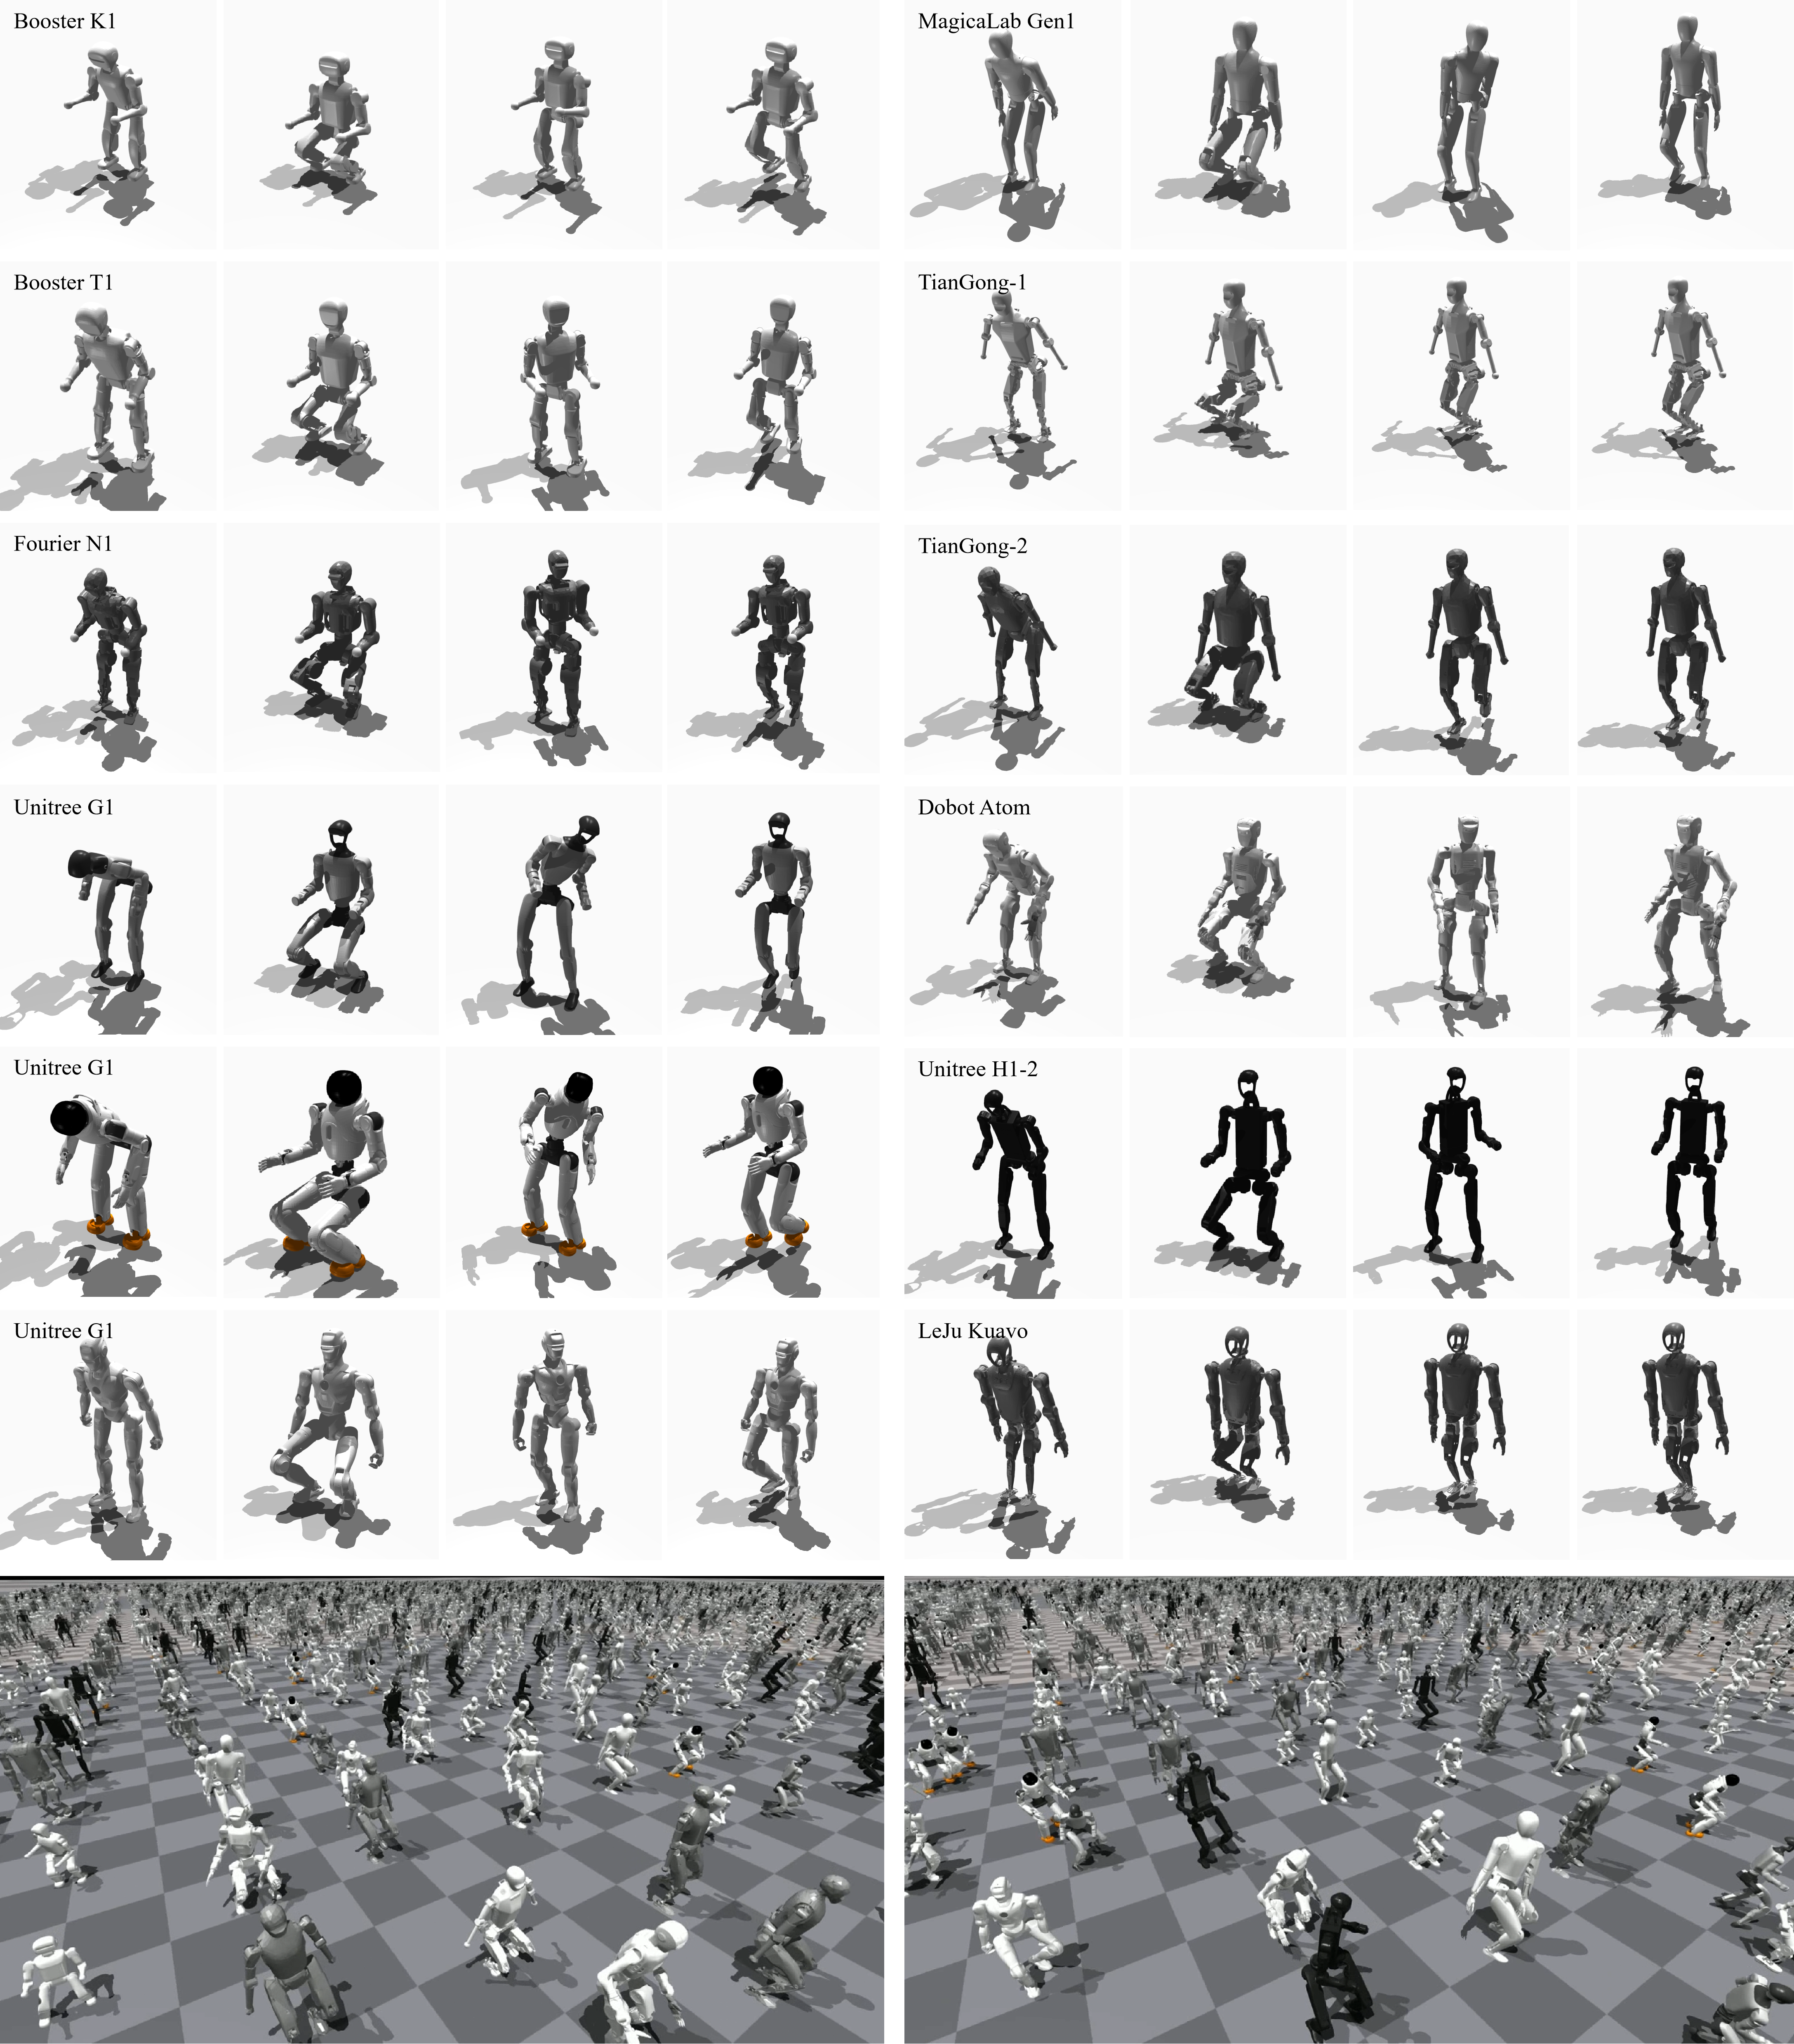
\includegraphics[width=0.95\linewidth]{images/simulation_experiment.png}
\caption{\small \textbf{Evaluation of 12 humanoid robots in simulation,} including Booster K1, Booster T1, Fourier N1, Unitree G1, Agibot X2, EngineAI PM01, MagicaLab Gen1, TianGong-1, TianGong-2, Dobot Atom, Unitree H1-2, and LeJu Kuavo. The first six rows report per-robot evaluations, while the final rows show parallel evaluations across all robots.}
\label{fig:simulation_experiment}
\end{figure*}

\begin{figure*}[htbp]
\centering
\includegraphics[width=0.95\linewidth]{images/embodiment data.pdf}
\caption{\small \textbf{Visualization of samples from procedurally generated embodiment data.}}
\label{fig:embodiment data}
\end{figure*}


